\documentclass[aspectratio=169]{beamer}
\usetheme{Madrid}
\usepackage[utf8]{inputenc}
\usepackage[T1]{fontenc}
\usepackage{tikz}
\usepackage{amssymb}
\usepackage{graphicx}
\setbeamertemplate{navigation symbols}{}
\setbeamercolor{title}{fg=white,bg=magenta!70!red}
\setbeamercolor{frametitle}{fg=white,bg=magenta!70!red}
\setbeamercolor{block title}{bg=magenta!70!red!20,fg=black}
\setbeamercolor{block body}{bg=magenta!70!red!8,fg=black}
\setbeamercolor{item}{fg=magenta!70!red}
\setbeamercolor{itemize item}{fg=magenta!70!red}
\setbeamertemplate{itemize item}[triangle]

\title{Foundations 7 — Flight Computer}
\subtitle{Loops, MOD, averages, sorting, and recursion --- real algorithmic thinking}
\author{ByteForge --- Grade 9 --- The Deep Diver}
\date{}

\begin{document}

\begin{frame}
    \titlepage
\end{frame}

\begin{frame}{Today's Missions}
    \Large
    \begin{itemize}
        \item First Transmission
        \item Countdown Log
        \item Fizz Report
        \item Average Fuel Reading
        \item Sort the Manifest
        \item Recursive Fuel Calculation
    \end{itemize}
\end{frame}

\begin{frame}{A loop that COMPUTES something, not just repeats}
    \large
    \begin{itemize}
        \item An accumulator: start a total at 0, add ONE more value each pass through the loop
        \item By the end, the total holds the sum of everything --- genuinely useful, not just repetition
    \end{itemize}
\end{frame}


\begin{frame}{MOD tests whether something divides evenly}
    \large
    \begin{itemize}
        \item \texttt{i \% 3 == 0} is true exactly when i is a multiple of 3 --- remainder 0
        \item Combine with OR to catch multiples of 3 OR 5, plus a counter
    \end{itemize}
\end{frame}


\begin{frame}{Bubble sort --- the classic, done for real}
    \large
    \begin{itemize}
        \item Compare NEIGHBOURING items, swap if they are the wrong way round
        \item Repeat enough passes and the largest values "bubble" to the end
        \item Simple to trace by hand --- genuinely why it is taught first
    \end{itemize}
\end{frame}


\begin{frame}{Recursion --- a function that calls ITSELF}
    \large
    \begin{itemize}
        \item Factorial(5) = 5 x Factorial(4), all the way down to Factorial(1) = 1
        \item That final Factorial(1) is the BASE CASE --- miss it and it never stops
    \end{itemize}
\end{frame}

\begin{frame}{Real-World Examples}
    \large
    \begin{itemize}
        \item A real rocket launch genuinely uses running totals (fuel remaining), threshold checks (abort if below X), and sorted telemetry data --- this chapter's ideas, for real.
        \item Sorting a leaderboard by score is bubble sort's exact job, just usually done by a faster algorithm at real scale.
    \end{itemize}
\end{frame}


\begin{frame}{Image}
    \begin{center}
    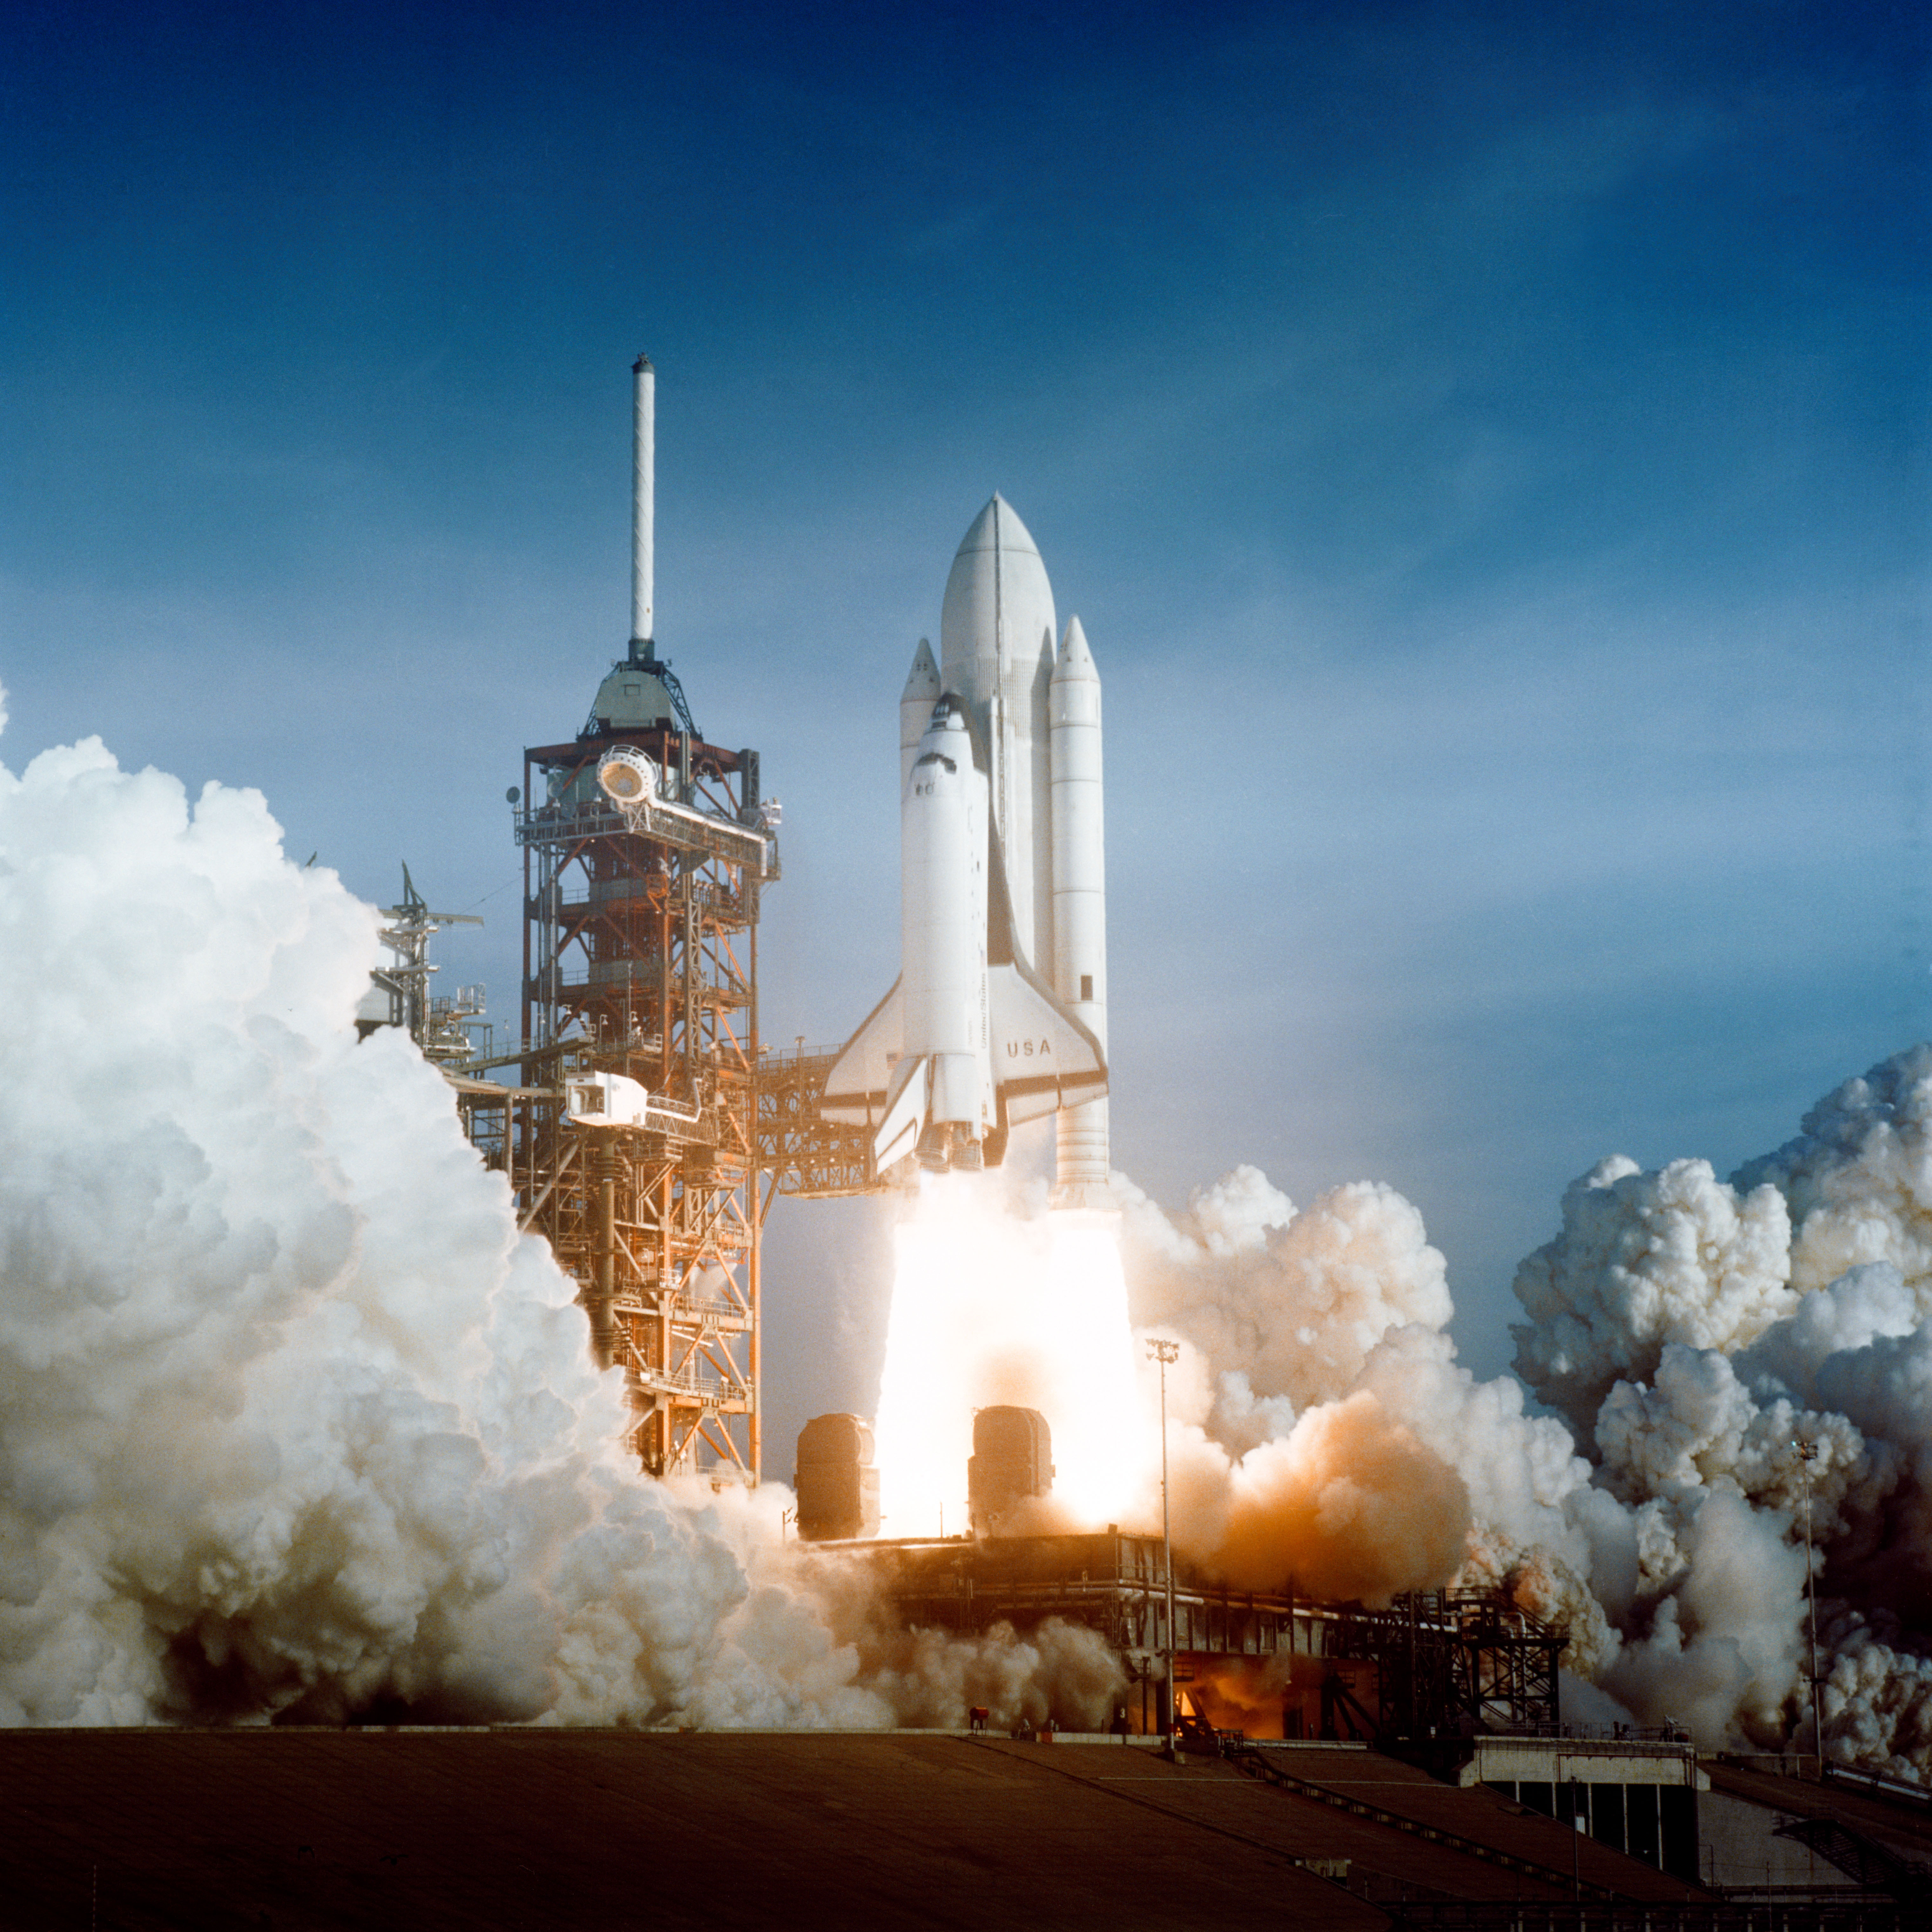
\includegraphics[width=0.5\textwidth]{images/rocket.jpg}

    \large A real flight computer runs on exactly this kind of algorithmic thinking --- loops, thresholds, sorting real sensor data.

    \small Space Shuttle launch --- NASA, public domain, via Wikimedia Commons
    \end{center}
\end{frame}

\begin{frame}{Let Them Discover}
    \large
    By hand, bubble-sort these 5 numbers on paper: 64, 34, 25, 12, 22. How many full passes did it take before nothing needed swapping?
\end{frame}

\begin{frame}{Your Turn}
    \Large
    Open the mission map, find \textbf{Foundations 7 — Flight Computer}, and fly it for real ---
    everything you just saw, you now do yourself.
\end{frame}

\end{document}
